\documentclass[conference]{IEEEtran}
\usepackage{url}
\usepackage{graphicx}
\usepackage{subfigure}

\begin{document}

\title{An exploration of pull-based software development on Github}

\author{\IEEEauthorblockN{Georgios Gousios and Martin Pinzger and Arie van
Deursen}
\IEEEauthorblockA{
Software Engineering Research Group\\
Delft University of Technology\\
Delft, The Netherlands\\
Email: \{g.gousios, m.pinzger, a.vandeursen\}@tudelft.nl}
}

\maketitle

\begin{abstract}
Foo
\end{abstract}

\begin{IEEEkeywords}
Git, pull request, collaborative development
\end{IEEEkeywords}

\section{Introduction}

Since its appearance in 2005, the Git version control system has revolutionized
the way distributed software development has been carried out. Driven by
pragmatic needs, Git was designed from scratch to work as an advanced patch
management system, rather than a versioned file system, the then dominant
version control system ({\sc vcs}) paradigm. In Git, a file is an ordered set of
changes, the serial application of which lead to the current file, and
consequently file tree, state. The changesets can originate from a local
filesystem or a remote host; Git tools facilitate the acquisition and
application of changesets on a local Git datastore. The distributed nature
of Git enables a pull-based development model, where changes are offered
to a project repository through a network of project forks; it is up to the
project repository owner to accept or reject the incoming pull requests.

Several code hosting sites, including Github and BitBucket, tapped on the
opportunity to make the pull-based development model more accessible to
programmers. A unique characteristic of such sites is that they allow any user
to fork any public repository. The clone creates a public project that belongs
to user that cloned it, so the user can modify the repository without being part
of the development team. What is more important is they automate the selective
contribution of commits from the clone to the source, through pull requests. As
mentioned earlier, pull requests are not unique to code hosting sites; in fact,
the Git software distribution includes the \textsf{git-request-pull} utility
which provides the same functionality at the command line. Github
improved\footnote{Not everyone agrees:
https://github.com/torvalds/linux/pull/17} this process significantly by
integrating code reviews, discussions and issues, thus effectively lowering the
entry barrier for casual contributions. Combined, cloning and pull requests
create a new development model, where changes are pushed to the project
maintainers and go through code review by the community before being integrated. 

In this paper, we provide a quantitative exploration of the way the pull-based
distributed software development model works on Github. Specifically, we examine
50 large Ruby and Java projects and identify common factors that affect pull
request handling and merge time. Our contributions are the following:

\begin{itemize}

  \item We define the pull-based contribution model

  \item We provide 

\end{itemize}

\section{Distributed development models}



\subsubsection{Shared repository} Developers share a common repository, with read
and write permissions. To work, they clone it locally, modify its contents,
potentially introducing new branches, and push their changes back to the central
one. To cope with multiple versions and multiple developers, larger projects
usually adopt a {\em branching model}. While the exact details depend on the
project requirements, usually branching models include feature branches, where
developers implement new features and fix bugs, and release branches, which
store the state of each project release. After the work has finished on the
feature branch its contents are merged appropriately to release branches and the
project master branch.

\subsubsection{Pull requests} The project repository is not shared among
developers; instead, developers fork (create an identical copy of) the
repository and make their changes independent of each other. When a set of
changes is ready to merge with the main repository, they create a pull request,
which specifies a branch and a list of commits to merge with a branch in the
main repository. The main repository owner is responsible to test the changes
and pull them to the project's master branch. 

\subsubsection{Intra-branch pull requests} As pull requests only specify branches
from which certain commits can be pulled, there is nothing that forbids their
use in the shared repository approach. In such cases, developers specify as the
source branch a branch in the same repository as the target one. Intra-branch
pull requests are usually accompanied by code reviews and discussion; this is
why they are primarily performed if the project tooling supports this kind of
interaction.



\section{Aspects of pull-based software development}

\subsection{Lifetime of pull requests}

\begin{figure*}
\centering
\subfigure[Percentage of pull requests that have been merged before being closed]{
  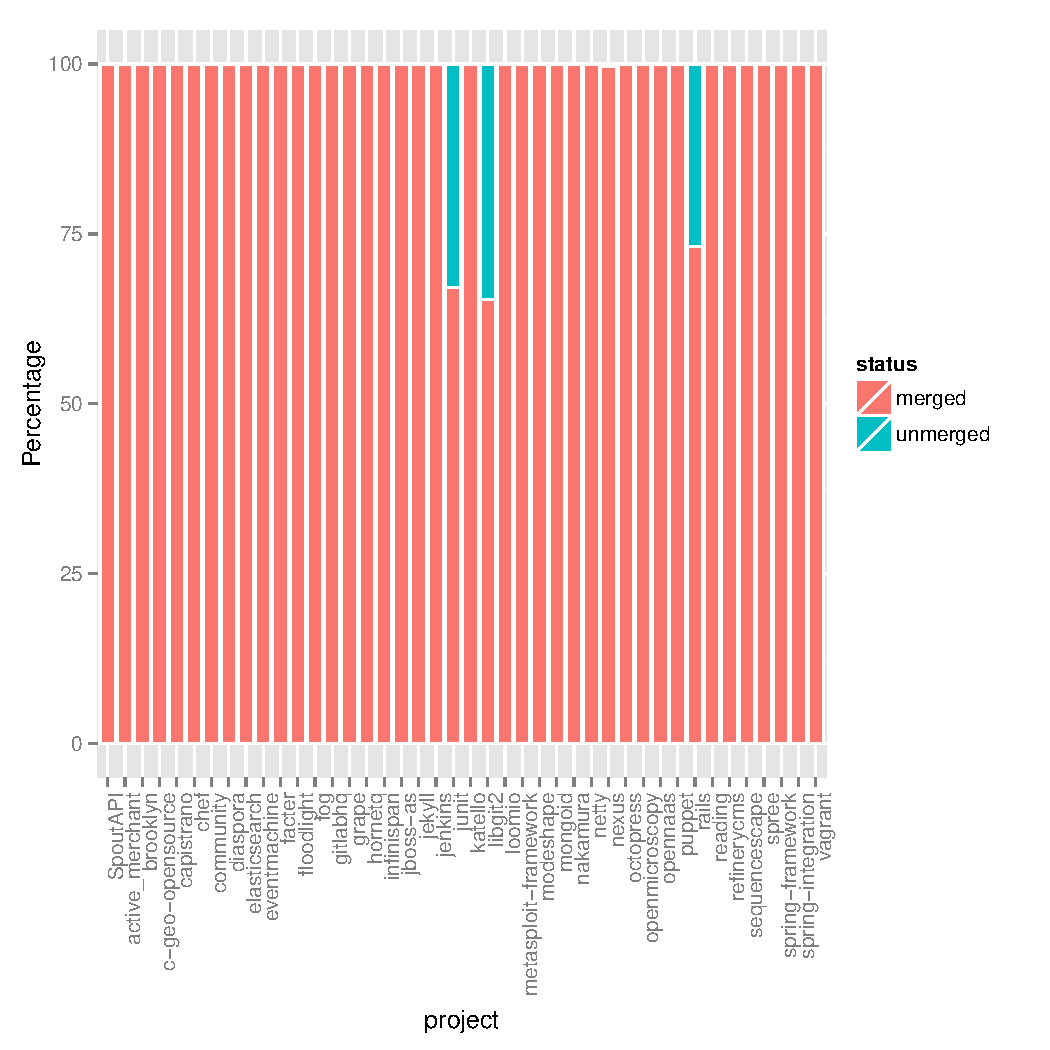
\includegraphics[scale=0.4]{perc-merged.pdf} 
  \label{fig:perc-merged}
}
\subfigure[Frequency distribution of lifetime for merged pull requests]{
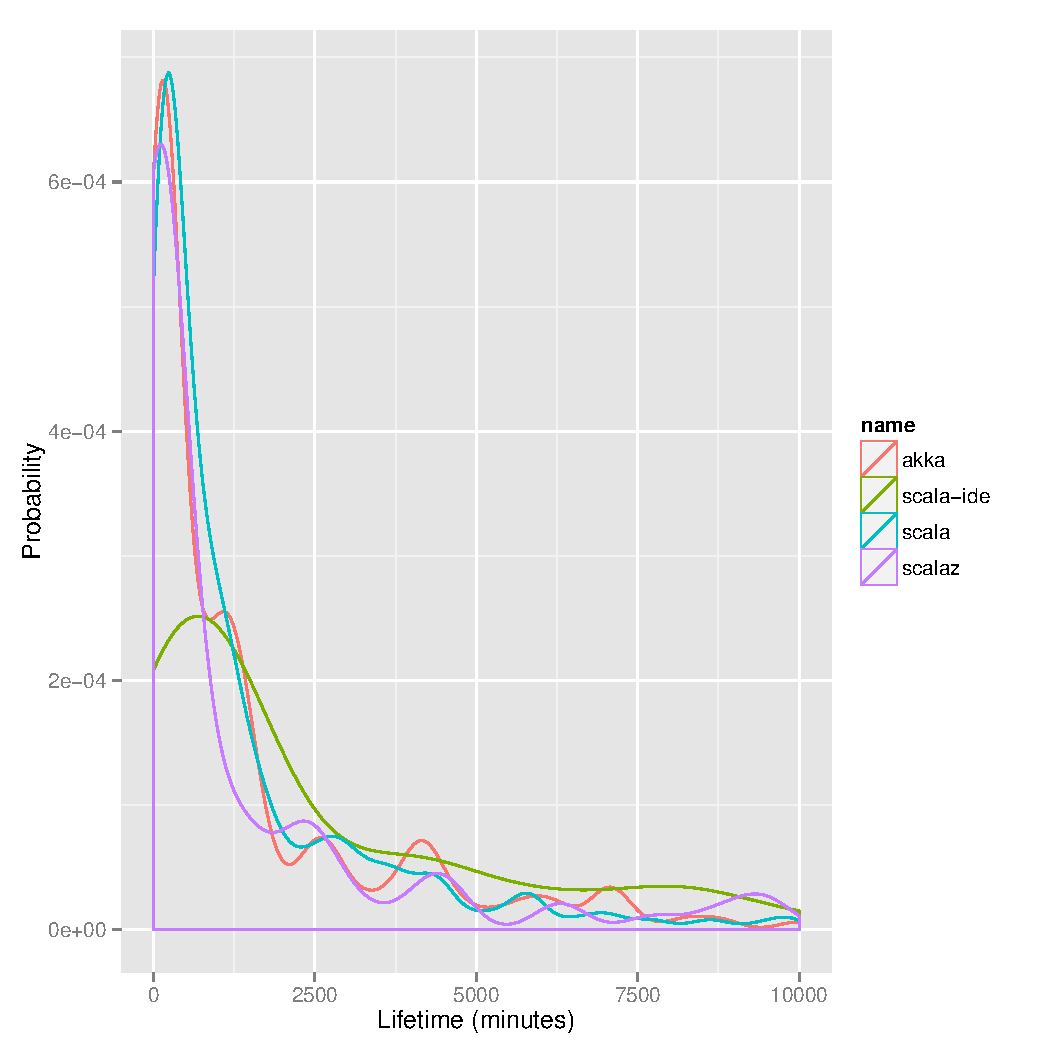
\includegraphics[scale=0.3]{lifetime-freq.pdf}
\label{fig:lifetime-freq}
}
\subfigure[Lifetime statistics for merged pull requests]{
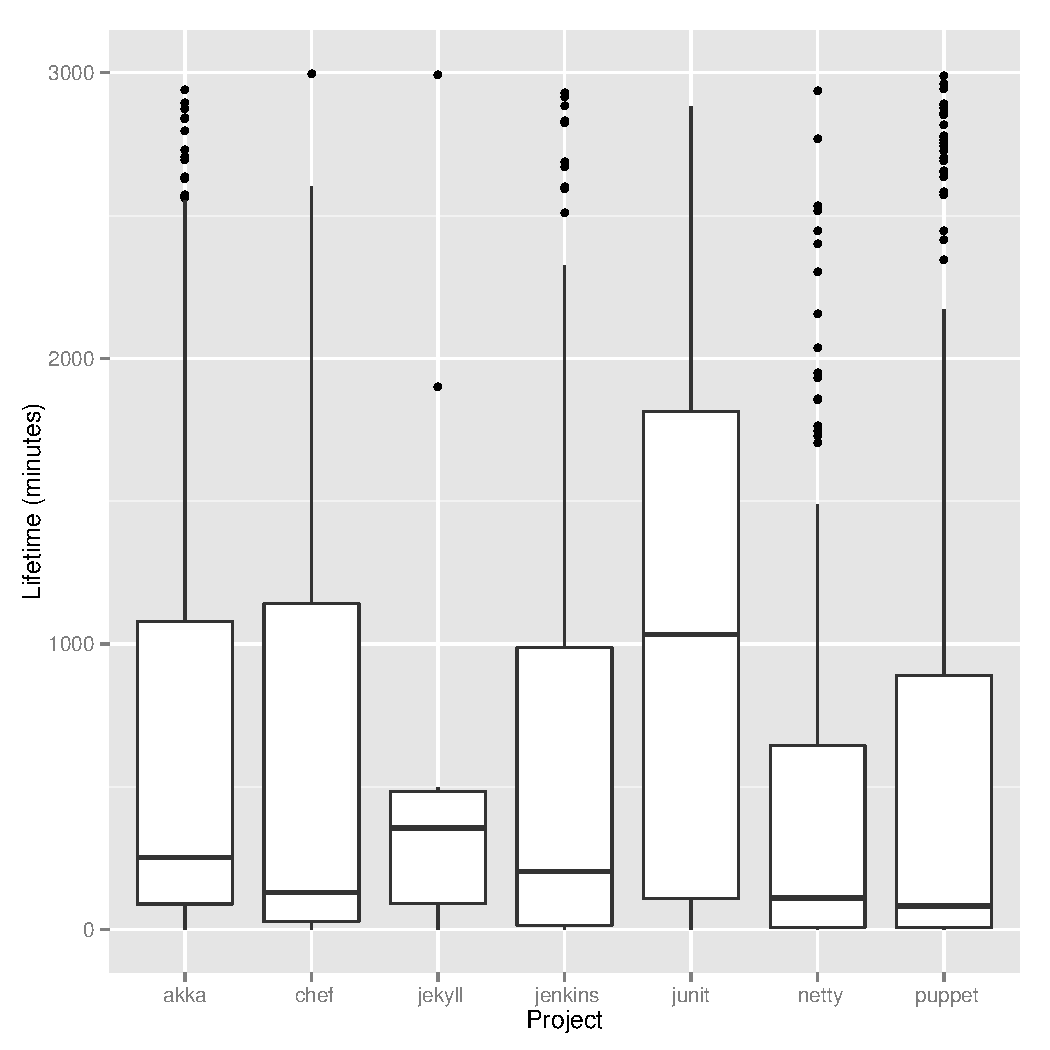
\includegraphics[scale=0.3]{lifetime-boxplot.pdf}
\label{fig:lifetime-boxplot}
}
\caption{Plots of pull request life time.}
\end{figure*}



An important observation is that there are several pull requests whose
lifetime is only limited to a ver

\subsection{Sizes for pull requests}



\subsection{Discussion and Code review}

\subsection{Team size}

\subsection{Testing}

\section{Acceptance and rejection}

\section{Discussions and Conclusion}

\section{Related Work}

\cite{Bird09}
\cite{Cornf10}
\cite{Dabbi12}
\cite{Bird12}
\cite{Barr12}
\cite{Buffe99}
\cite{Mens02}
\cite{Shiha12}

Global software development
\section{Conclusions}

\section*{Acknowledgements}
This work is partially supported by Marie Curie {\sc ief} 298930 -- {\sc sefunc}.

\bibliographystyle{ieeetr}
\bibliography{pullreqs}

\end{document}
